% Intended LaTeX compiler: xelatex
\documentclass[aspectratio=64,12pt]{beamer}
\usepackage{graphicx}
\usepackage{longtable}
\usepackage{wrapfig}
\usepackage{rotating}
\usepackage[normalem]{ulem}
\usepackage{amsmath}
\usepackage{amssymb}
\usepackage{capt-of}
\usepackage{hyperref}
\institute{Università di Siena}
\usepackage{localheader}
\usepackage{tikz}
\usepackage{booktabs,tabularx,tabularray}
\usepackage{setspace}
\usepackage{quoting}
\usepackage[italian]{babel}
\usepackage{fancybox}
\usepackage{tabularray}
\usetheme{default}
\author{Massimo D'Antoni}
\date{2024-2025}
\title{L'analisi normativa dell'intervento pubblico: mercati ed efficienza}
\subtitle{Scienza delle Finanze}
\hypersetup{
 pdfauthor={Massimo D'Antoni},
 pdftitle={L'analisi normativa dell'intervento pubblico: mercati ed efficienza},
 pdflang={Italian}}
\begin{document}

\maketitle

%%%%%%%%%%%%%%%%%%%%%%%%%%%%%%%%%%%%%%%%%%%%
\begin{frame}{Perché l'intervento dello Stato?}
\begin{itemize}
\item Alla domanda possiamo rispondere da un’ottica:
\begin{itemize}
\item \alert{positiva};
\item \alert{normativa}.
\end{itemize}
\item L’adozione di un’ottica normativa richiede un criterio di valutazione. Tradizionalmente: 
\begin{itemize}
\item \alert{equità};
\item \alert{efficienza};
\end{itemize}
entrambi sono obiettivi desiderabili, ma la definizione di efficienza è meno controversa.
\end{itemize}
\end{frame}

\section{L'efficienza}


%%%%%%%%%%%%%%%%%%%%%%%%%%%%%%%%%%%%%%%%%%%%
\begin{frame}{Efficienza ed equità}
\begin{itemize}
\item Guardiamo agli \alert{effetti}, alle \alert{conseguenze}, che un'azione o politica determina per gli individui della collettività.
\item Parlando di \alert{efficienza} valutiamo e ordiniamo i diversi esiti evitando confronti tra individui. \item Riferendoci all'\alert{equità} confrontiamo e pesiamo gli effetti sui diversi individui.
\item \alert{Efficienza paretiana} (criterio proposto da Vilfredo Pareto, 1848-1923): è efficiente in senso paretiano e rappresenta un «ottimo paretiano» una situazione a partire dalla quale non è possibile migliorare l’utilità di nessuno senza peggiorare quella di qualcun altro.
\end{itemize}
\end{frame}

%%%%%%%%%%%%%%%%%%%%%%%%%%%%%%%%%%%%%%%%%%%%
\begin{frame}{Efficienza paretiana}
\begin{itemize}
\item L’efficienza paretiana può essere definita a partire dal criterio di «dominanza paretiana»:
\begin{itemize}
\item A «domina» B (è preferibile in senso paretiano a B) se nessun individuo preferisce B ad A e almeno un individuo preferisce A a B.
\item In una versione più debole del criterio: se tutti gli individui preferiscono A a B.\\[1mm]
\end{itemize}
\item Il criterio dell'efficienza è molto parsimonioso in quanto non richiede informazioni sull’intensità delle preferenze dei diversi individui.
\item L'efficienza è sempre in funzione dell'insieme degli esiti possibili.
\begin{itemize}
\item Date le preferenze degli individui, un esito può cessare di essere efficiente se aumentiamo l’insieme di esiti disponibili, può diventare efficiente se riduciamo tale insieme
\end{itemize}
\end{itemize}
\end{frame}

%%%%%%%%%%%%%%%%%%%%%%%%%%%%%%%%%%%%%%%%%%%%
\begin{frame}{Un esempio: individuiamo gli esiti efficienti}
\begin{columns}
\begin{column}{.5\columnwidth}
\begin{itemize}
\item Consideriamo 5 possibili esiti e due individui:
\begin{itemize}
\item Individuo 1: A > B > C > D > E
\item Individuo 2: E > B > C > A > D
\end{itemize}
\item Verifichiamo se un esito è dominato, cioè se esiste un altro esito ad esso preferito da entrambi gli individui.
\item Un esito non dominato è efficiente.
\item In questo caso, gli esiti C e D sono dominati da altri esiti
\item Gli esiti efficienti sono E, B e A.
\end{itemize}
\end{column}

\begin{column}{.5\columnwidth}
\footnotesize
Potremmo assegnare dei valori numerici 
coerenti con gli ordinamenti e rappresentare
le opzioni graficamente:

\begin{center}
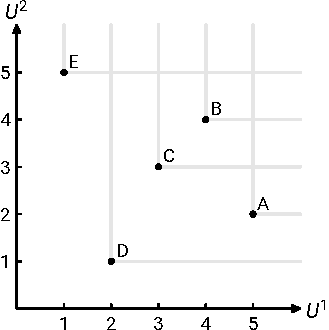
\includegraphics[width=\textwidth]{./figure/efficienza-1.pdf}
\end{center}
\end{column}
\end{columns}
\end{frame}

%%%%%%%%%%%%%%%%%%%%%%%%%%%%%%%%%%%%%%%%%%%%
\begin{frame}{Alcune osservazioni sulla nozione di efficienza}
\begin{itemize}
\item Il concetto di efficienza evita i confronti interpersonali.
\item Nella tradizione dell’utilitarismo del XIX secolo era ritenuto desiderabile ciò che aumenta l’utilità complessiva di una collettività. L’utilitarismo classico considerava astrattamente possibile confrontare l’aumento di utilità di un individuo con la riduzione dell’utilità di un altro individuo.
\item A partire dagli anni ‘30 del XX secolo si è affermata una visione critica, che ha rifiutato l’idea che le utilità siano confrontabili.
\item Senza confrontare le variazioni di utilità non è possibile rispondere a domande come «quanto è intensa la preferenza di A rispetto a B per l’individuo 1 se confrontata con la preferenza di B rispetto ad A dell’individuo 2?»
\end{itemize}
\end{frame}

%%%%%%%%%%%%%%%%%%%%%%%%%%%%%%%%%%%%%%%%%%%%
\begin{frame}{Alcune osservazioni sulla nozione di efficienza /2}
\begin{itemize}
\item Il criterio paretiano consente di effettuare confronti basandosi esclusivamente sulla conoscenza del fatto che per un ciascun individuo A è meglio/peggio di B
\item Si tratta di un criterio che, quando rispettato, risulta coerente con altri più esigenti criteri:
\begin{itemize}
\item il criterio della maggioranza: se A è Pareto superiore a B, allora A sarà preferito a B a maggioranza
\item il criterio utilitarista: se A è Pareto superiore a B, vuol dire che l’utilità di tutti gli individui aumenta (o non diminuisce), quindi anche l’utilità totale aumenta
\end{itemize}
\item Ci sono molti casi nei quali il criterio non ci fornisce una risposta, anche quando a noi tale risposta appare ovvia:
  \begin{itemize}
  \item come valutiamo una politica che toglie 100€ a un individuo
    povero per aumentare di 10€ il reddito di un individuo ricco?
  \item Cosa dire del caso in cui diamo 1000€ a un individuo ricco e non diamo nulla ad altri individui più poveri?
  \end{itemize}
\end{itemize}
\end{frame}

%%%%%%%%%%%%%%%%%%%%%%%%%%%%%%%%%%%%%%%%%%%%
\begin{frame}{L'efficienza potenziale e il test di compensazione}
\begin{itemize}
\item Consideriamo un cambiamento dello status quo che determina un vantaggio considerevole per un numero elevato di individui al prezzo di uno svantaggio modesto per pochi individui (al limite uno solo).
\begin{itemize}
\item Il cambiamento non è un miglioramento paretiano
\item \ldots{}eppure ci appare desiderabile!
\end{itemize}
\item Kaldor e Hicks negli anni '30 del XX secolo hanno proposto di uscire da questa impasse immaginando un’ipotetica compensazione monetaria tra «vincenti» e «perdenti».
\item Il test di compensazione effettua un confronto tra guadagni e perdite quantificandoli in termini monetari.
\end{itemize}
\end{frame}


%%%%%%%%%%%%%%%%%%%%%%%%%%%%%%%%%%%%%%%%%%%%
\begin{frame}{L'efficienza potenziale e il test di compensazione /2}
\begin{itemize}
\item Nella versione di Kaldor:
\begin{itemize}
\item chiediamo ai perdenti quale somma monetaria potrebbe compensarli dell’adozione del cambiamento proposto;
\item chiediamo ai vincenti se essi continuerebbero a desiderare il cambiamento anche qualora dovessero pagare ai perdenti una compensazione pari alla cifra da questi indicata;
\item se la risposta è positiva, il cambiamento supera il test ed è socialmente desiderabile
\end{itemize}
\item Nella versione di Hicks:
\begin{itemize}
\item chiediamo ai vincenti quale somma monetaria potrebbe compensarli della mancata adozione del cambiamento proposto
\item chiediamo ai perdenti se essi sarebbero disposti a pagare la somma indicata dai vincenti per evitare il cambiamento che li danneggia
\item se la risposta è \alert{negativa}, il cambiamento supera il test ed è socialmente desiderabile.
\end{itemize}
\end{itemize}
\end{frame}

%%%%%%%%%%%%%%%%%%%%%%%%%%%%%%%%%%%%%%%%%%%%
\begin{frame}{Il test di compensazione in formule}
\begin{itemize}
\item In formule:
\begin{itemize}
\item Poniamo che l’utilità di $i$ dipenda da una certa azione $X\in\{A, B\}$ del governo e dal
reddito $R^i$: $U^i(X, R^i)$,
\item se nel passaggio da B ad A l’individuo 1 è un vincente e l’individuo 2 è
un perdente abbiamo:
$U^1(A, R^1) > U^1(B, R^1)$ e $U^2(A, R^2) < U^2(B, R^2)$
\item esisteranno dunque due somme $Y^1$ e $Y^2$ (dette variazioni compensative) tali che
\begin{equation*}
U^1(A, R - Y^1) = U^1(B, R^1) \qquad U^2(A, R + Y^2) = U^2(B, R^2)
\end{equation*}
\item il test di Kaldor è soddisfatto se $Y^1 >  Y^2$
\end{itemize}
\item Per esercizio, trovate le formule corrispondenti per il criterio di Hicks, che utilizza le variazioni equivalenti
\item I due criteri differiscono perché la somma che sono disposto a pagare per ottenere un cambiamento che mi avvantaggia (variazione compensativa) non coincide in generale con la somma che sono disposto ad accettare per rinunciarvi (variazione equivalente).
\end{itemize}
\end{frame}

%%%%%%%%%%%%%%%%%%%%%%%%%%%%%%%%%%%%%%%%%%%%
\begin{frame}{Il test di compensazione: osservazioni}
\begin{itemize}
\item Il test di compensazione non richiede che la compensazione abbia effettivamente luogo (se così fosse avremmo un miglioramento paretiano). È sufficiente che essa sia \alert{ipoteticamente} possibile.
\begin{itemize}
\item Se la valutazione non ha luogo, a essere svantaggiato potrebbe essere un individuo con reddito più basso\dots
\item Ci convince come criterio di valutazione?
\end{itemize}
\item Proprio perché variazioni equivalenti e compensative non sono uguali, A potrebbe essere meglio di B secondo Kaldor (Hicks) ma non secondo Hicks (Kaldor).
\item Possono anche aver luogo dei paradossi: 
\begin{itemize}
\item Potrebbe accadere che, secondo uno dei due criteri, A è meglio di B e contemporaneamente B è meglio di A!
\end{itemize}
\end{itemize}
\end{frame}

%%%%%%%%%%%%%%%%%%%%%%%%%%%%%%%%%%%%%%%%%%%%
\begin{frame}{L'efficienza potenziale nell'analisi economica}
\begin{itemize}
\item Quando gli economisti parlano di una soluzione «più efficiente», spesso fanno riferimento all’efficienza potenziale più che all’efficienza paretiana.
\item Essi intendono dire che si è determinata una situazione a partire dalla quale, con un opportuno schema di trasferimenti monetari, è possibile ottenere un miglioramento paretiano.
\item In questo modo, si separano le considerazioni di efficienza (la «dimensione della torta» aumenta) da quelle equitative (come la maggiore torta viene divisa tra le parti), rimandando implicitamente queste ultime a un momento logicamente successivo.
\end{itemize}
\end{frame}

\section{Efficienza e mercati nel modello neoclassico}

%%%%%%%%%%%%%%%%%%%%%%%%%%%%%%%%%%%%%%%%%%%%
\begin{frame}{L'efficienza in un'economia di beni privati}
\begin{itemize}
\item \alert{Beni privati} = è possibile escludere altri dal consumo (escludibilità) e il
mio consumo rende impossibile il consumo dello stesso bene da parte di altri
(rivalità)
\begin{itemize}
\item La rivalità implica: $X = x^1 + x^2 + \dots + x^n$
\end{itemize}
\item Un esito è un'\alert{allocazione}, cioè una descrizione di quanto ciascun individuo
consuma di ciascun bene.
\item Se nell’economia non c’è produzione (economia di «puro scambio») possiamo
ricorrere alla «scatola di Edgeworth»
\end{itemize}
\end{frame}

%%%%%%%%%%%%%%%%%%%%%%%%%%%%%%%%%%%%%%%%%%%%
\begin{frame}{Allocazioni efficienti nella scatola di Edgeworth}
\begin{columns}
\begin{column}{.5\columnwidth}
\fontsize{11}{11}\selectfont
\begin{itemize}
\item 2 individui (1 e 2) e 2 beni (X e Y)
\item A meno che le curve di indifferenza siano tangenti, l’allocazione è inefficiente in quanto dominata da allocazioni preferite da entrambi (ad es. allocazione B).
\item La condizione di tangenza delle curve di indifferenza caratterizza dunque le allocazioni efficienti (ad es. allocazione A)
\item Formalmente la condizione di tangenza
tra curve di indifferenza: $\text{SMS}^1_{XY}=\text{SMS}^2_{XY}$.
\end{itemize}
\end{column}
\begin{column}{.5\columnwidth}
\footnotesize

\begin{figure}
\centering
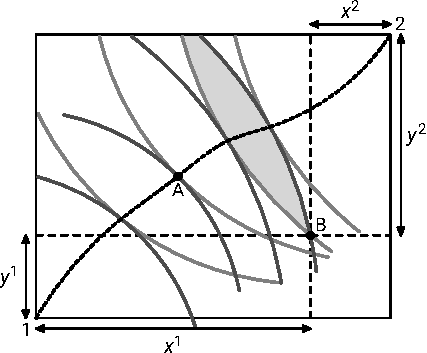
\includegraphics[height=4cm]{./figure/edgeworth-1.pdf}
\end{figure}

Il saggio marginale di sostituzione (SMS) rappresenta l’inclinazione della curva di indifferenza. 
\end{column}
\end{columns}
\end{frame}

%%%%%%%%%%%%%%%%%%%%%%%%%%%%%%%%%%%%%%%%%%%%
\begin{frame}{Allocazioni efficienti nella scatola di Edgeworth /2}
\begin{columns}
\begin{column}{.5\columnwidth}
\begin{figure}
\centering
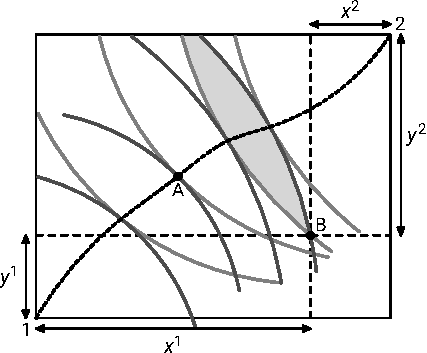
\includegraphics[height=5cm]{./figure/edgeworth-1.pdf}
\end{figure}
\end{column}

\begin{column}{.5\columnwidth}
\begin{itemize}
\item La soluzione efficiente realizza il massimo di utilità di un individuo data l’utilità dell’altro individuo.
\item Ci sono infinite allocazioni efficienti (sulla «curva dei contratti»).
\item Spostandosi da una allocazione efficiente all’altra si migliora la condizione di uno dei due individui a spese dell’altro.
\item Nota bene: l’allocazione efficiente A non è Pareto superiore all’allocazione inefficiente B
\end{itemize}
\end{column}
\end{columns}
\end{frame}

%%%%%%%%%%%%%%%%%%%%%%%%%%%%%%%%%%%%%%%%%%%%
\begin{frame}{Un'economia con produzione}
\begin{columns}
\begin{column}{.5\columnwidth}
\begin{itemize}
\item Nel caso più semplice: un input (lavoro, L) che può essere allocato alla
produzione di due beni X e Y:
\begin{equation*}
X = f_X(L_X)\quad  Y = f_Y(L_Y)\quad L = LX + LY
\end{equation*}
\item La \alert{frontiera delle
possibilità di produzione} è concava per effetto dei rendimenti
decrescenti.
\item L’inclinazione della frontiera è il SMT (\alert{saggio marginale di trasformazione}), pari al rapporto tra i costi marginali di produzione dei due beni
\begin{equation*}
\text{SMT}_{XY}=\frac{\text{CMg}_X}{\text{CMg}_Y}
\end{equation*}
\end{itemize}
\end{column}


\begin{column}{.5\columnwidth}
\begin{figure}[htbp]
\centering
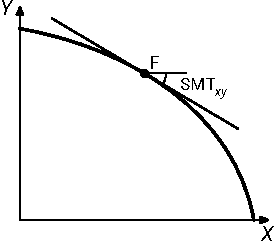
\includegraphics[height=5cm]{./figure/frontiere-1.pdf}
\end{figure}
\end{column}
\end{columns}
\end{frame}

%%%%%%%%%%%%%%%%%%%%%%%%%%%%%%%%%%%%%%%%%%%%
\begin{frame}{Efficienza con produzione}
\begin{columns}
\begin{column}{.5\columnwidth}
\begin{itemize}
\item L’efficienza nello scambio e nella produzione è individuata dalla condizione:
\begin{equation*}
\text{SMT}^1_{XY}=\text{SMT}^2_{XY}=\text{SMT}_{XY}
\end{equation*}
\end{itemize}
\end{column}

\begin{column}{.5\columnwidth}
\begin{figure}[htbp]
\centering
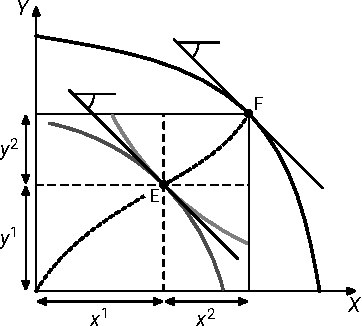
\includegraphics[height=5cm]{./figure/edgeworth-2.pdf}
\end{figure}
\end{column}
\end{columns}
\end{frame}

%%%%%%%%%%%%%%%%%%%%%%%%%%%%%%%%%%%%%%%%%%%%
\begin{frame}{Frontiera del benessere}
\begin{columns}
\begin{column}{.5\columnwidth}
\begin{itemize}
\item Date le risorse disponibili e la tecnologia:
\item fissato un livello minimo di utilità per un individuo ($U^2$)
\item la soluzione efficiente individua il massimo livello di utilità ottenibile dall’altro individuo ($U^1$).
\item Ci sono dunque molteplici soluzioni efficienti, una per ciascun livello $U^2$.
\item Le combinazioni di utilità dei due individui così determinate individuano nello spazio delle utilità la cosiddetta \alert{frontiera del benessere}.
\end{itemize}
\end{column}
\begin{column}{.5\columnwidth}
\begin{figure}[htbp]
\centering
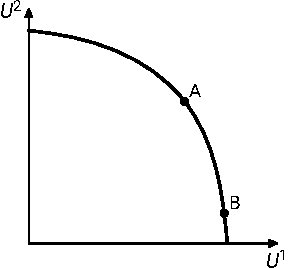
\includegraphics[height=5cm]{./figure/frontiere-2.pdf}
\end{figure}
\end{column}
\end{columns}
\end{frame}

\section{I teoremi fondamentali dell'economia del benessere}


%%%%%%%%%%%%%%%%%%%%%%%%%%%%%%%%%%%%%%%%%%%%
\begin{frame}{Primo teorema fondamentale dell’economia del benessere}
Supponiamo che:
\begin{itemize}
\item tutte le interazioni avvengano su mercati concorrenziali;
\item l’utilità degli individui sia determinata esclusivamente dal consumo dei beni
acquistati tramite interazioni di mercato;
\item mercati concorrenziali = gli individui sono \emph{price taker}, non hanno la
possibilità di influenzare i prezzi con le loro decisioni;
\item sulla base dei prezzi di mercato gli individui formulano i propri piani di
consumo (e quindi di acquisto/vendita);
\item il mercato rende compatibili tali piani: i prezzi di mercato si modificano
fino ad eguagliare domanda e offerta di ciascun bene.
\end{itemize}
\begin{block}{}
L’allocazione ottenuta in corrispondenza di un equilibrio di mercato concorrenziale è efficiente in senso paretiano (o anche: rappresenta un ottimo paretiano).
\end{block}
\end{frame}


%%%%%%%%%%%%%%%%%%%%%%%%%%%%%%%%%%%%%%%%%%%%
\begin{frame}{Primo teorema fondamentale dell’economia del benessere /2}
\begin{columns}
\begin{column}{.5\columnwidth}
In un equilibrio di mercato concorrenziale le curve di indifferenza degli individui sono tangenti

\begin{figure}[htbp]
\centering
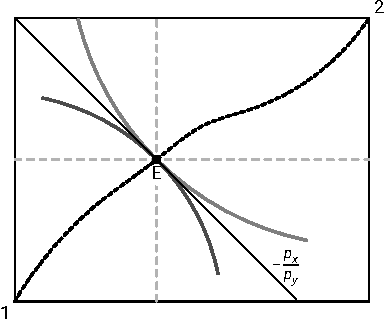
\includegraphics[height=5cm]{./figure/edgeworth-4.pdf}
\end{figure}
\end{column}

\begin{column}{.5\columnwidth}
\begin{figure}[htbp]
\centering
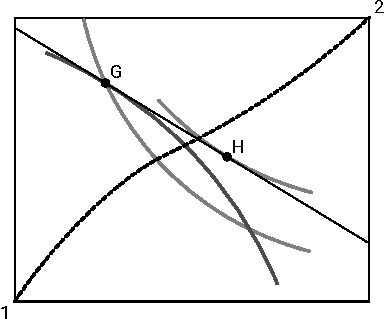
\includegraphics[height=5cm]{./figure/edgeworth-5.pdf}
\end{figure}
\small
In G, dove le curve di indifferenza non sono tangenti, non può esserci equilibrio di mercato concorrenziale. Infatti, se i prezzi rendono ottimo G per 2, l’ottimo per 1 sarà in un punto differente, H.
\end{column}
\end{columns}
\end{frame}

%%%%%%%%%%%%%%%%%%%%%%%%%%%%%%%%%%%%%%%%%%%%
\begin{frame}{Una spiegazione intuitiva del I teorema fondamentale}
\begin{itemize}
\item Un altro modo per illustrare il risultato del I teorema, utilizzando le condizioni al margine:
\begin{itemize}
\item Se gli individui sono \emph{price taker}, fisserano il paniere ottimale in corrispondenza del punto in cui
\end{itemize}
\begin{equation*}
\text{SMS}^1_{XY}=\frac{p_X}{p_Y} \qquad \text{SMS}^2_{XY}=\frac{p_X}{p_Y}
\end{equation*}
\begin{itemize}
\item Se tutti scambiano sulla base degli stessi prezzi: $\text{SMS}^1_{XY} = \text{SMS}^2_{XY}$.
\end{itemize}
\item Considerando anche la produzione:
\begin{itemize}
\item un’impresa concorrenziale fissa la propria quantità in corrispondenza del punto in cui:   $\text{CMg}_X=p_X$
\item da cui: $$\text{SMT}_{XY}=\frac{\text{CMg}_X}{\text{CMg}_Y}=\frac{p_X}{p_Y} = \text{SMS}^i_{XY}$$
\end{itemize}
\end{itemize}
\end{frame}

%%%%%%%%%%%%%%%%%%%%%%%%%%%%%%%%%%%%%%%%%%%%
\begin{frame}{La rilevanza pratica del I teorema fondamentale}
\begin{itemize}
\item Il teorema formalizza quanto già Adam Smith aveva teorizzato con la metafora
della «mano invisibile».
\item Il teorema evidenzia le condizioni necessarie per l'esito
  dell'interazione di mercato sia desiderabile. Il teorema non sarà verificato
  quando:
\begin{itemize}
\item sono presenti beni che non hanno le caratteristiche di beni privati
(rivalità ed escludibilità);
\item i mercati non sono \alert{concorrenziali}
\item alcune interazioni non passano attraverso i mercati (\alert{esternalità})
\item la presenza di \alert{asimmetrie informative} impedisce scambi
  mutuamente vantaggiosi.
\end{itemize}
\item In questi casi si parla di «fallimenti del mercato».
\end{itemize}
\end{frame}

%%%%%%%%%%%%%%%%%%%%%%%%%%%%%%%%%%%%%%%%%%%%
\begin{frame}{Secondo teorema fondamentale dell'economia del benessere}
\begin{block}{}
Sotto ipotesi di convessità delle preferenze e della tecnologia, qualsiasi allocazione efficiente è ottenibile come equilibrio di mercato. 
\end{block}
\begin{itemize}
\item Presa una qualsiasi allocazione efficiente E, esiste un insieme di prezzi e
una distribuzione iniziale delle risorse tali che l’allocazione di
equilibrio è E.
\item Dunque, non solo gli equilibri di mercato concorrenziale sono un
sottoinsieme dell’insieme delle allocazioni efficienti (come afferma il I
teorema). Il teorema afferma che ogni elemento dell’insieme degli
ottimi paretiani è ottenibile come equilibrio di mercato.
\end{itemize}
\end{frame}


%%%%%%%%%%%%%%%%%%%%%%%%%%%%%%%%%%%%%%%%%%%%
\begin{frame}{Secondo teorema fondamentale dell'economia del benessere /2}
\begin{columns}
\begin{column}{.45\columnwidth}
\begin{itemize}
\item Riformuliamo il teorema: data una qualsiasi allocazione efficiente E e una qualsiasi distribuzione iniziale delle risorse A, è sempre possibile, mediante un opportuno trasferimento di risorse, ottenere E come equilibrio di mercato.
\item Per raggiungere E non c’è necessità di interferire con il meccanismo dei prezzi, basta un trasferimento, da effettuarsi «a monte» del sistema di mercato.
\end{itemize}
\end{column}

\begin{column}{.55\columnwidth}
\begin{figure}
\centering
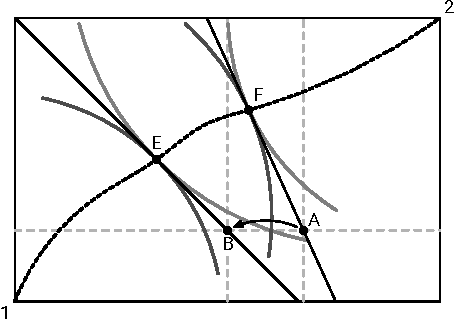
\includegraphics[height=5cm]{./figure/edgeworth-6.pdf}
\end{figure}
\end{column}
\end{columns}
\end{frame}


%%%%%%%%%%%%%%%%%%%%%%%%%%%%%%%%%%%%%%%%%%%%
\begin{frame}{Secondo teorema fondamentale: l'ipotesi di convessità}
\begin{columns}
\begin{column}{.45\columnwidth}
\small
\begin{itemize}
\item Quando non abbiamo convessità delle preferenze o della tecnologia la soluzione efficiente potrebbe non essere ottenibile come equilibrio di mercato:
\item nella figura, abbiamo ipotizzato preferenze non convesse per l’individuo 1;
\item l’allocazione E è efficiente, ma non esistono prezzi in grado di ottenere tale allocazione come equilibrio di mercato.
\end{itemize}
\end{column}

\begin{column}{.55\columnwidth}
\begin{figure}
\centering
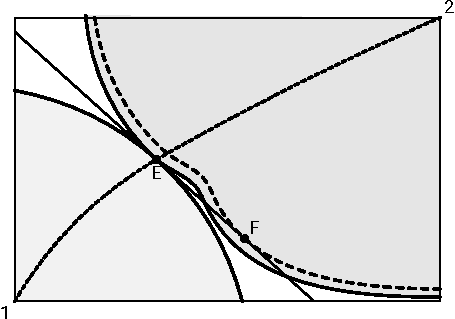
\includegraphics[height=5cm]{./figure/edgeworth-7.pdf}
\end{figure}
\end{column}
\end{columns}
\end{frame}


%%%%%%%%%%%%%%%%%%%%%%%%%%%%%%%%%%%%%%%%%%%%
\begin{frame}{La rilevanza pratica del II teorema fondamentale}
\begin{itemize}
\item Qual è l’effettiva portata del secondo teorema fondamentale?
\item È possibile conseguire qualsiasi allocazione efficiente operando una redistribuzione delle dotazioni iniziali senza interferire con i prezzi determinati da mercati concorrenziali.
\item  Esiste nella realtà qualcosa di analogo alle «dotazioni iniziali» del modello di equilibrio economico generale, cui commisurare le imposte?
\item \alert{Imposta in somma fissa} (\emph{lump sum tax}): imposte il cui ammontare non dipende dalle decisioni individuali.
\item Tra le imposte «reali» con le quali è possibile redistribuire, nessuna ha le caratteristiche di un’imposta in somma fissa.
\item Anche il secondo teorema fondamentale va inteso come una \alert{costruzione astratta e ideale}, che individua le condizioni per un’ideale separazione tra la dimensione dell’efficienza (lasciata al mercato) e quella dell’equità (responsabilità dello Stato).
\end{itemize}
\end{frame}

%%%%%%%%%%%%%%%%%%%%%%%%%%%%%%%%%%%%%%%%%%%%
\begin{frame}{La giustificazione dell'intervento pubblico: una sintesi}
\begin{itemize}
\item L'analisi economica spiega come il mercato sia in grado di coordinare in
modo efficiente l'attività economica degli individui, fornendo incentivi e
guidandone le scelte (la «mano invisibile»)
\item Il mercato come meccanismo di organizzazione sociale è insufficiente e non
vive nel vuoto istituzionale: è necessario un quadro di norme e di garanzie per
l'esercizio dei diritti di proprietà da parte degli individui.
\item \alert{«Fallimenti del mercato»}: circostanze in cui l'esito del mercato non è
efficiente e può (almeno astrattamente) essere migliorato da un intervento
correttivo dello Stato:
\begin{itemize}
\item esternalità
\item beni «pubblici», che il mercato non garantisce in quantità adeguata
\item mercati non concorrenziali (in particolare: monopoli naturali)
\item mercati incompleti o mancanti (in particolare: mercati assicurativi,
mercati con asimmetrie informative)
\end{itemize}
\item Il mercato non garantisce l'\alert{equità distributiva}.
\end{itemize}
\end{frame}

%%%%%%%%%%%%%%%%%%%%%%%%%%%%%%%%%%%%%%%%%%%%
\begin{frame}{A sua volta anche l'intervento dello Stato è soggetto a «fallimenti»}
\begin{itemize}
\item L'azione di governo, anche quando ben orientata, soffre le conseguenze di
limitazioni informative;
\item i limiti dei meccanismi di scelta collettiva possono portare a decisioni che
non riflettono le preferenze dei membri della collettività;
\item chi deve eseguire le decisioni pubbliche potrebbe perseguire obiettivi
diversi da quelli della collettività;
\item gli attori economici possono distogliere risorse dalle attività produttive e
impiegarle per condizionare a proprio favore l’azione del governo (\emph{rent
seeking});
\item l'azione del governo può interferire negativamente con l'azione del mercato,
provocando distorsioni e inefficienze.
\begin{itemize}
\item ESEMPIO: le imposte e i sussidi necessari per realizzare una più equa
distribuzione possono scoraggiare l'attività economica.
\end{itemize}
\end{itemize}
\end{frame}

\end{document}
